\documentclass[12pt]{article}
\usepackage[utf8]{inputenc}
\usepackage{mathpazo}
\usepackage{subfig}
\usepackage[a4paper,top=3cm,bottom=3cm,left=2.5cm,right=2.5cm,marginparwidth=3cm]{geometry}
\pagestyle{myheadings}	\usepackage{tabularx}

% Paquetes
\usepackage{mathtools, amsmath, setspace, amsfonts, enumitem, listings}
\usepackage{cancel, amssymb, xfrac, enumitem, setspace, tcolorbox}
\usepackage{pdfpages, soul, graphicx, multicol, float}
\tcbuselibrary{theorems}

% Bibliography
\usepackage[spanish]{babel}
\usepackage[natbibapa]{apacite}
\bibliographystyle{apacite}

\usepackage[natbibapa]{apacite}
\bibliographystyle{apacite}

% Hipervinculos
\definecolor{udesa}{HTML}{00529B}
\usepackage[colorlinks=true, allcolors=udesa]{hyperref}
\usepackage{listings}
\usepackage[colorinlistoftodos]{todonotes}
\usepackage{parskip}

\DeclareMathOperator*{\plim}{plim}
\setlength{\parskip}{1em}

% Commands
\providecommand{\abs}[1]{\lvert#1\rvert}
\providecommand{\abs}[1]{\lvert#1\rvert}
\newcommand{\HRule}{\rule{\linewidth}{0.3mm}} 

\hypersetup{breaklinks=true,
            pdfauthor={Riquelme y Pacheco},
            pdftitle={Problem Set 5},
            colorlinks=true,
            citecolor=udesa,
            urlcolor=udesa,
            linkcolor=udesa,
            pdfborder={0 0 0}}


\markboth{4444}{Herramientas computacionales para la investigaci\'on - MAE UdeSA 2022}

\title{ %
\includegraphics[scale=0.5]{Logos/Udesa_Azul.jpg}\\
%\vspace{0.5cm}
Herramientas computacionales para la investigaci\'on \\
\vspace{0.3cm}
\textbf{Tarea 2: Data visualization}}
\author{Tom\'as Pacheco y Abigail Riquelme}
\date{Fecha de entrega: 31/07/2022}

\begin{document}
\maketitle
\onehalfspace


La segunda tarea de esta semana tiene como objetivo que confeccionemos un mismo mapa de tres formas distintas. 
Lo que vamos a mostrar es la cantidad de robos cada 1000 habitantes para la ciudad de Londres, desagregado por barrio. Como se dijo, la \'unica diferencia que tienen los mapas es que fueron hechos de distintas maneras en cuanto a paquetes. La Figura (\ref{crimggplot}) muestra el mapa hecho con \texttt{ggplot2} en R, la Figura (\ref{crimtmap}) muestra el mapa hecho con el paquete \texttt{tmap} en R y la Figura (\ref{crimstata}) muestra el mapa hecho con \texttt{spmap} en Stata.

\begin{figure}[H]
    \centering
    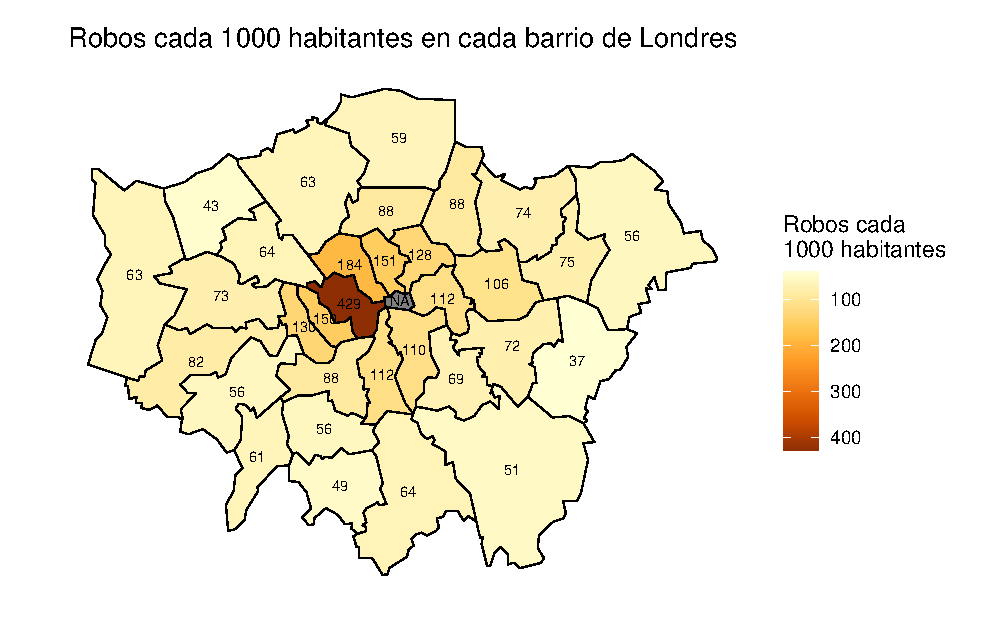
\includegraphics[width = \textwidth]{graficos/mapa_ggplot.eps}
    \caption{Mapa realizado con \texttt{ggplot} (R)}
    \label{crimggplot}
\end{figure}

\begin{figure}[H]
    \centering
    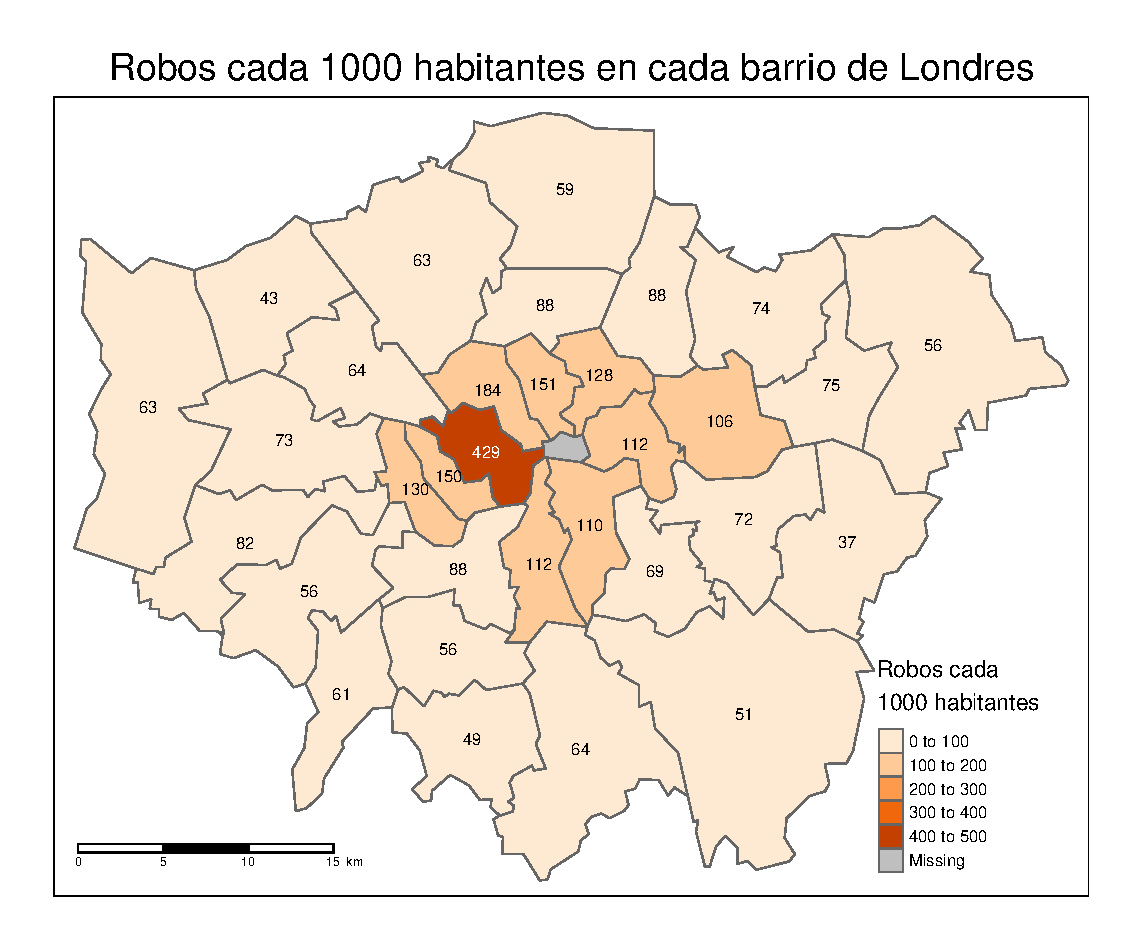
\includegraphics[width = \textwidth] {graficos/mapa_tmap.eps}
    \caption{Mapa realizado con \texttt{tmap} (R)}
    \label{crimtmap}
\end{figure}

Como se puede observar en estos dos mapas, los robos cada 1.000 habitantes son mayores en el centro de la ciudad. Se muestra que Westminster es el barrio con mayor criminalidad, con aproximadamente 429 cr\'imenes cada 1.000 habitantes. En las \'areas perif\'ericas de la ciudad, se observa una menor cantidad de cr\'imenes. En el centro se puede ver un barrio, City of London, con el que no contamos con informaci\'on. La escala del gr\'afico es un gradiente que toma colores claros para los valores menores y colores oscuros para los valores mayores. 

\begin{figure}[H]
    \centering
    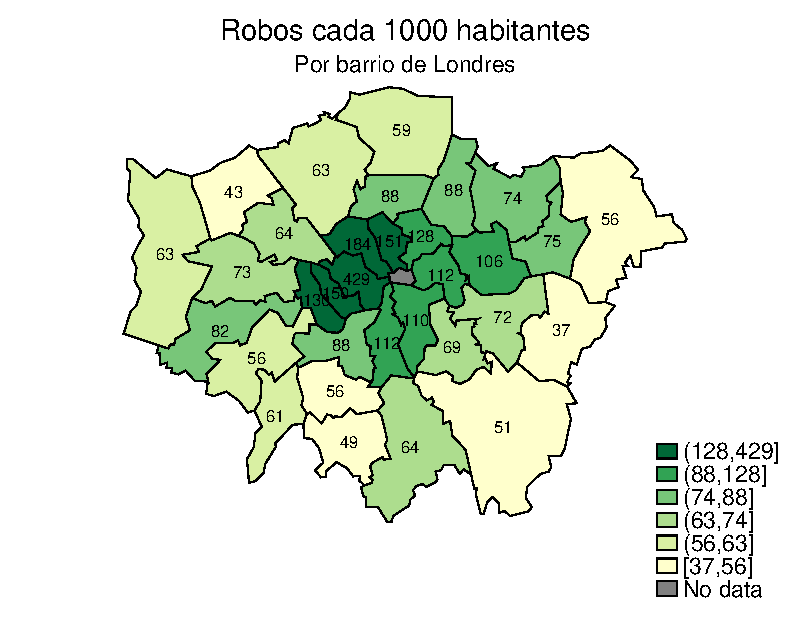
\includegraphics[width = \textwidth]{graficos/mapa_stata.eps}
    \caption{Mapa realizado con \texttt{spmap} (Stata)}
    \label{crimstata}
\end{figure}

Las conclusiones para este mapa en t\'erminos de la distribuci\'on de los cr\'imenes es exactamente igual a los anteriores. La \'unica diferencia es que la escala est\'a dividia en seis cuantiles. Gracias a esta divisi\'on, se puede apreciar un tanto mejor el hecho de que la mayor cantidad de cr\'imenes se concentran en torno al centro de la ciudad. 


\end{document}




